% !TEX TS-program = Xelatex
% !TEX encoding = UTF-8 Unicode

\documentclass[UTF8]{ctexart}
\usepackage{amsmath}
\usepackage[bottom]{footmisc}
\usepackage{geometry}
\usepackage{graphicx}
\usepackage{figsize}
\usepackage[separate-uncertainty = true,per-mode=symbol]{siunitx}
\usepackage{tabu}
\usepackage{wasysym}
\geometry{left=0.7in,right=0.7in,bottom=0.7in,top=0.7in}

\title{实验二十五:动态法测定铝的热导率}
\author{朱寅杰 1600017721}
\date{2018年5月18日}

\begin{document}

\maketitle
\setcounter{section}{25}

\subsection{峰谷测量}
热水端进水量\SI{750}{mL/min}、冷水端进水量\SI{600}{mL/min}
\begin{center}
\begin{tabu}{X[c,-1]|X[c,-1]X[c,-1]X[c,-1]X[c,-1]X[c,-1]X[c,-1]X[c,-1]X[c,-1]}
\hline
\#&1&2&3&4&5&6&7&8\\
\hline
峰:$t/$s&4061.36 &4068.45 &4074.65 &4080.86 &4087.95 &4092.38 &4103.9 &4110.99
\\
$U/$mV&726.32 &655.52 &596.92 &543.21 &488.28 &440.67 &397.95 &361.33
\\
\hline
谷1:$t$/s&4155.30 &4163.28 &4170.37 &4178.34 &4187.21 &4193.41 &4203.16 &4209.36
\\
$U/$mV&596.92 &563.96 &531.01 &494.38 &452.88 &415.04 &378.42 &346.68
\\
\hline
谷2:$t$/s&3976.28 &3984.25 &3989.57 &3996.66 &4005.52 &4011.73 &4023.25 &4032.11
\\
$U/$mV&598.14 &565.19 &532.23 &495.61 &454.10 &416.26 &379.64 &347.90
\\
\hline
\end{tabu}
\end{center}
最小二乘出来,斜率分别是\SI{6.96(25)}{\s}、\SI{7.81(11)}{\s}、\SI{7.87(29)}{\s}。相关系数写在各个图上了。算出热导率$\kappa=v^2c\rho T/4\pi$分别是\SI{270(9)}{W/mK}、\SI{241(4)}{W/mK}、\SI{239(9)}{W/mK}。
\begin{figure}[h]
  \centering
  \SetFigLayout{1}{3}
  \subfigure[]{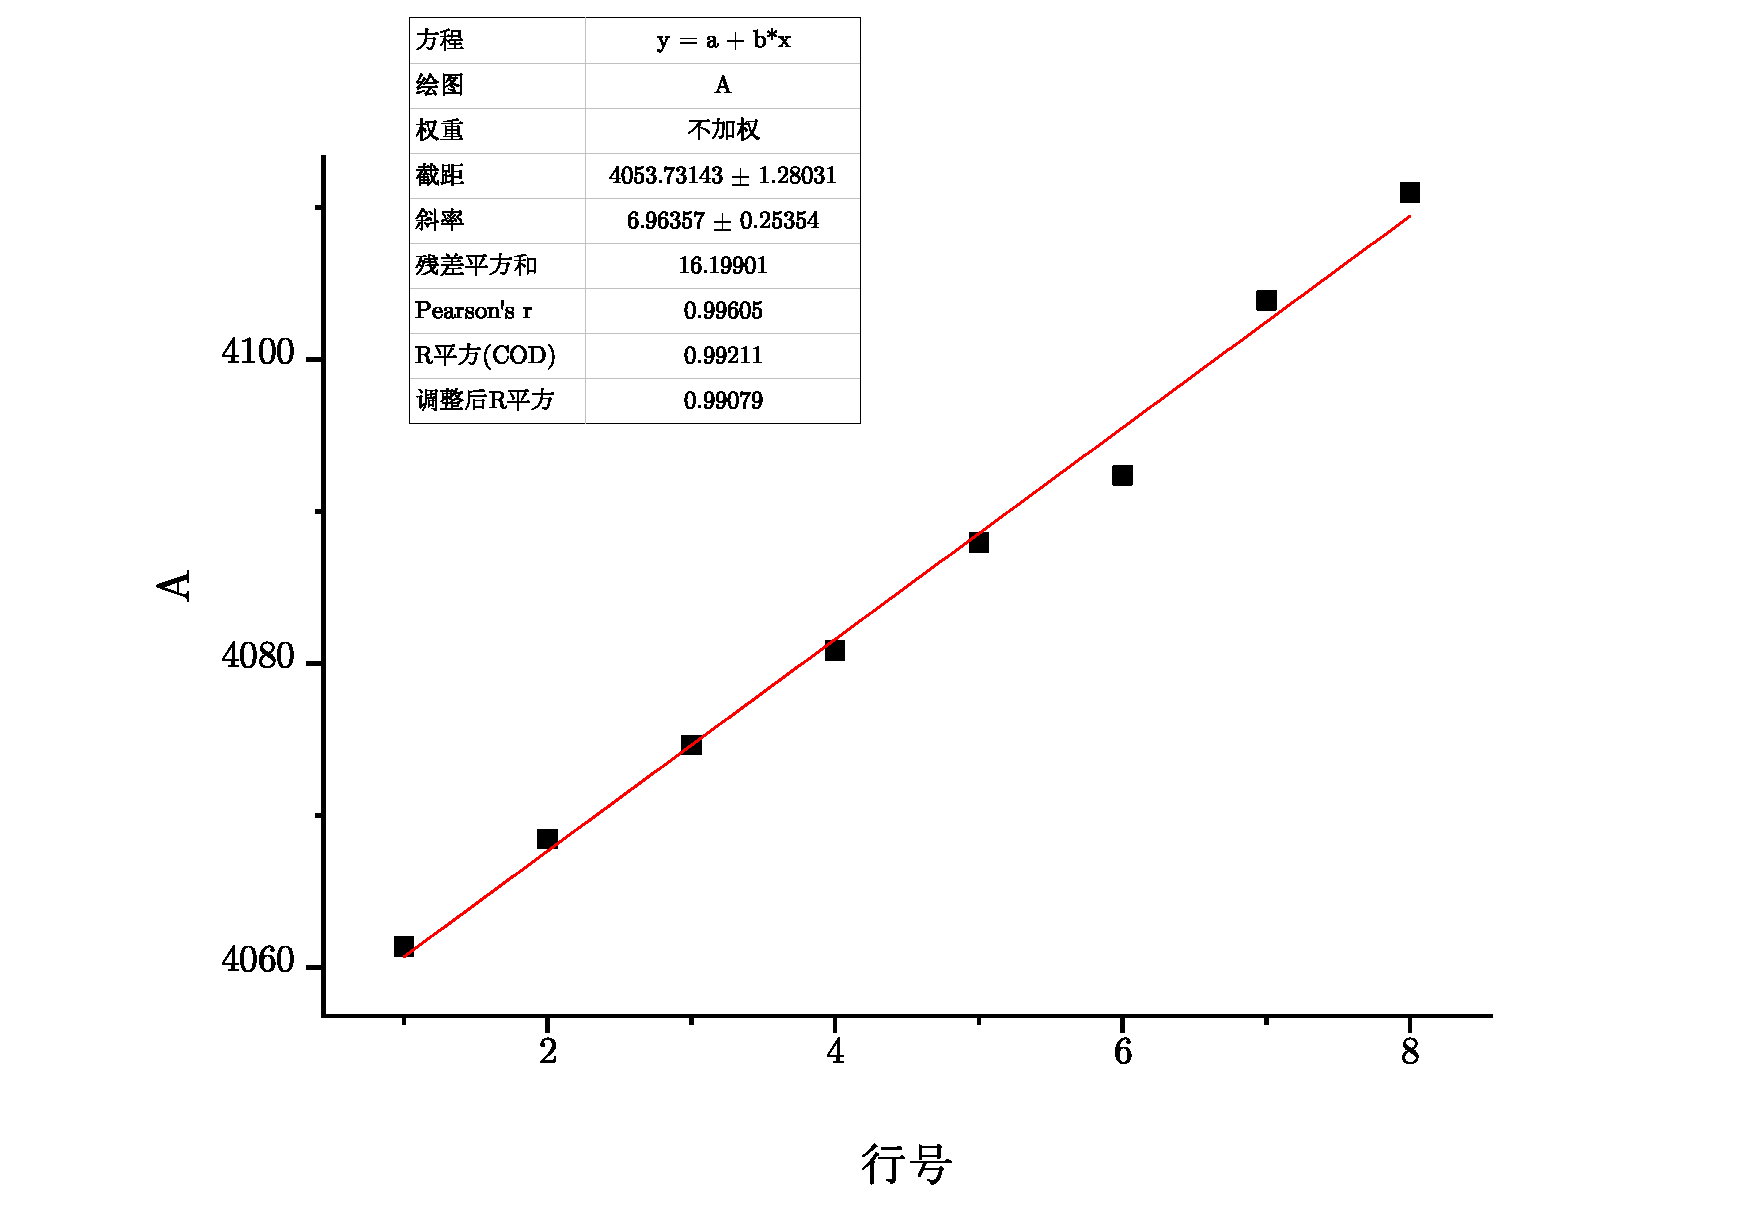
\includegraphics[width=0.33\linewidth]{feng.eps}}\hfill
  \subfigure[]{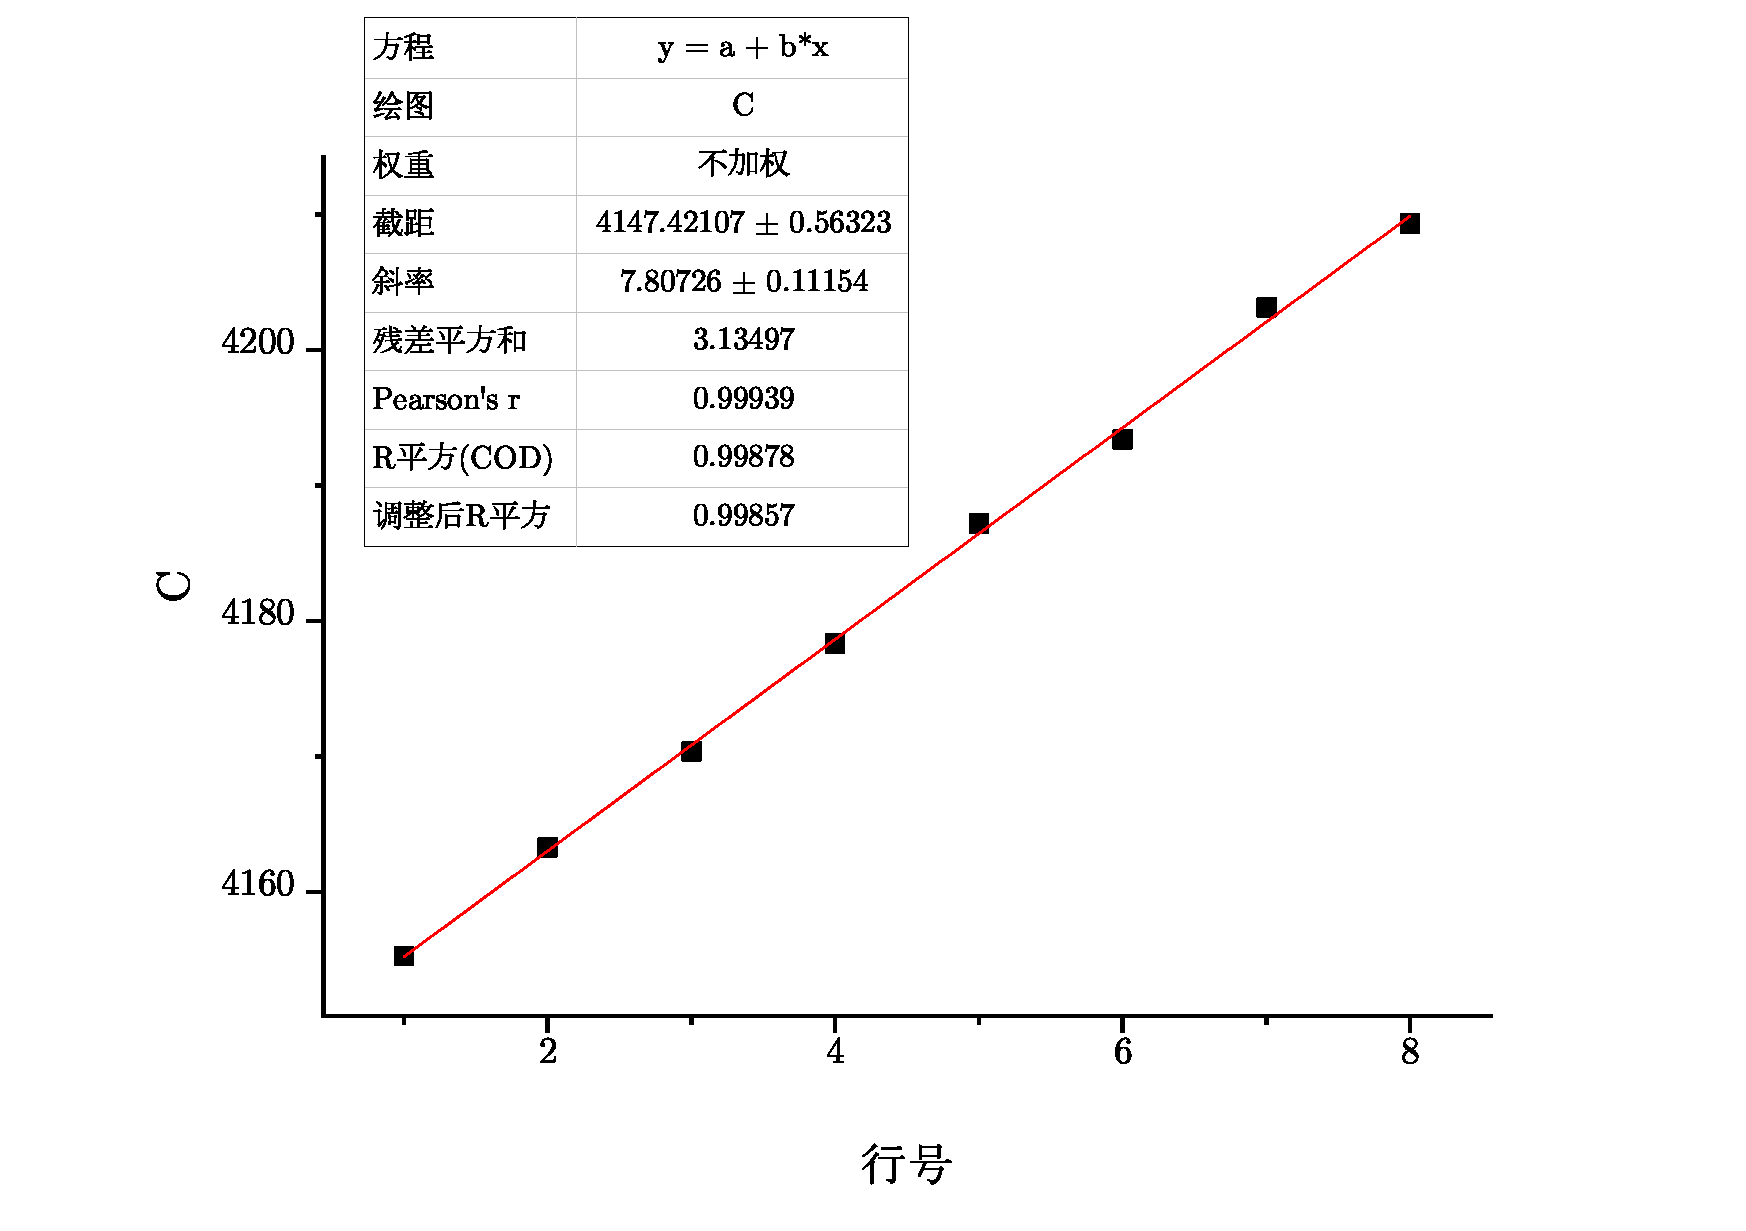
\includegraphics[width=0.33\linewidth]{gu1.eps}}\hfill
  \subfigure[]{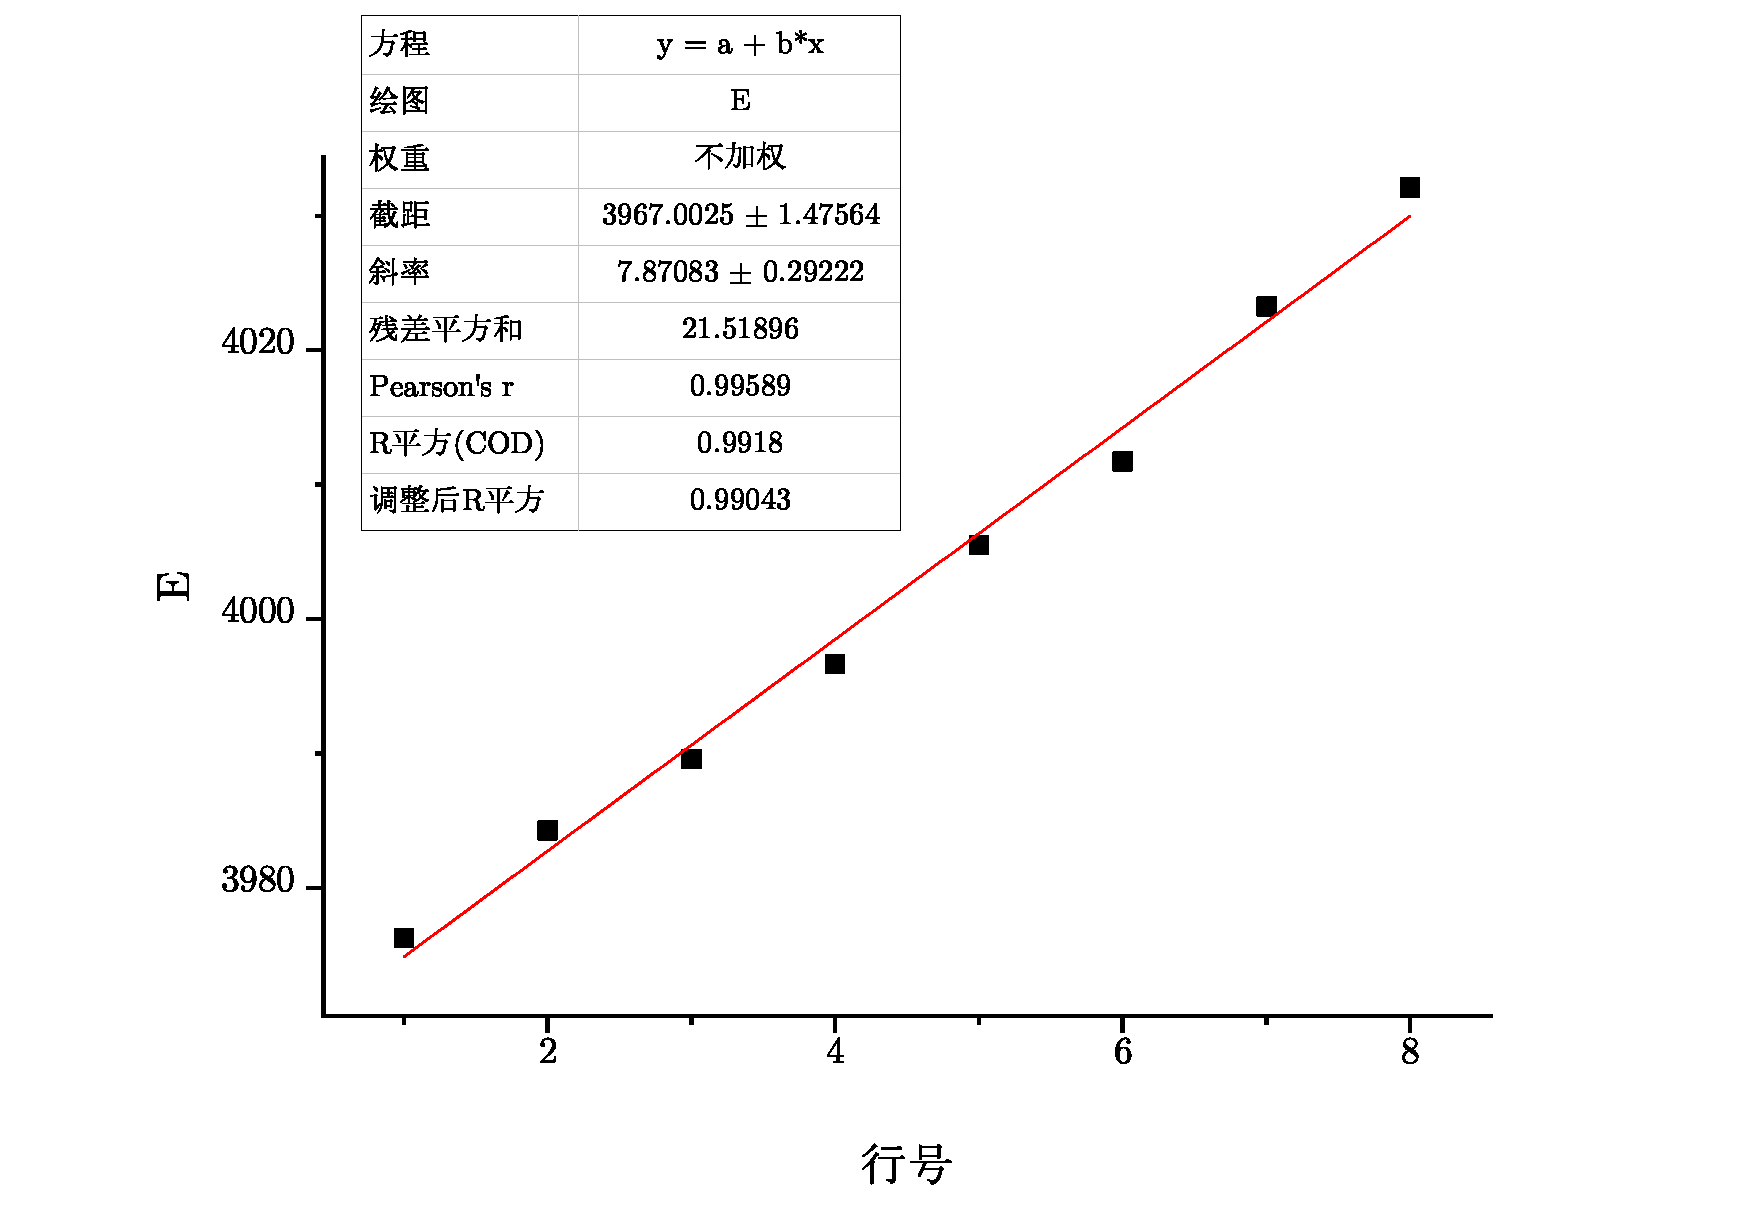
\includegraphics[width=0.33\linewidth]{gu2.eps}}\\
\end{figure}

如果用自制正弦拟合的软件,那出来分别是\SI{257.9}{W/mK}、\SI{244.61}{W/mK}、\SI{248.58}{W/mK}。
\subsection{思考题}
式25.5中第一项$T_0-kx$是静态下棒上两端起了温度差以后建立起的温度梯度,第二项是一个行波项乘上一个随距离的指数衰减,代表从一端激发的一个沿着棒传播的带有衰减的行波振动模式。

本实验条件下,由于棒上温度传感器的位置是固定的,因此无法实现对棒上各位置温度的连续监测,只能实现对某几个固定位置温度随时间变化的监测。所以测波长还是比测波速困难很多的。

把波速的测量转化为时间的测量,观察相位的延迟并且直接打在电脑屏幕上多直观啊是不。

观察到连续几个峰谷的位置保持稳定。测得的数据连续五组峰峰值的变化不超过2\%。
\end{document} 